\documentclass[tikz, convert=pdf2svg]{standalone}
\usetikzlibrary{shapes.geometric}
\usetikzlibrary{shapes.symbols}
\usetikzlibrary{shapes.arrows}
\begin{document}
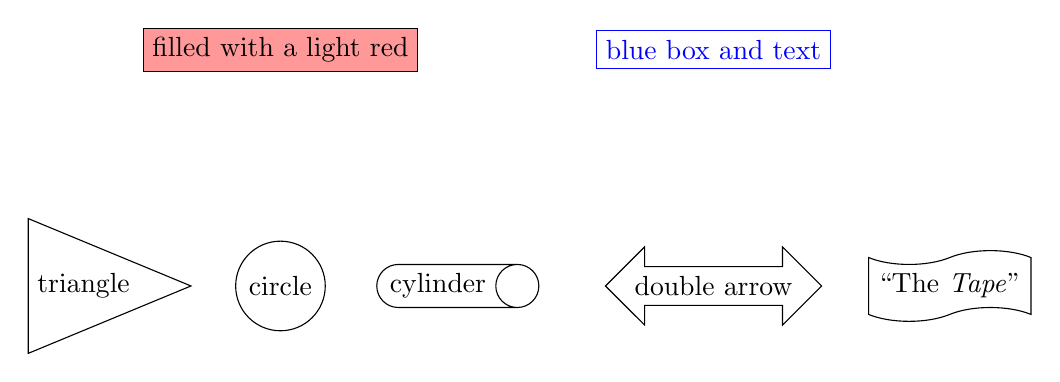
\begin{tikzpicture}
    \node[draw, isosceles triangle] (triangle) at (0,0)  {triangle};
    \node[draw, circle] (triangle) at (2.5,0)  {circle};
    \node[draw, cylinder] (cylinder) at (4.5,0)  {cylinder};
    \node[draw, shape=double arrow] (double arrow) at (8,0)  {double arrow};
    \node[draw, shape=tape] (tape) at (11,0)  {``The \textit{Tape}''};

    \node[draw, fill=red!40] (red) at (2.5,3) {filled with a light red};
    \node[draw, blue] (blue) at (8,3) {blue box and text};
\end{tikzpicture}
\end{document}
